\begin{figure*}[t]
\centering
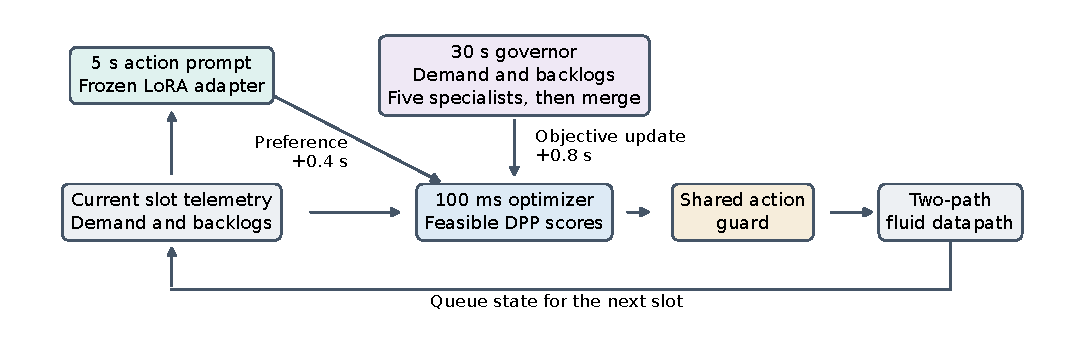
\includegraphics[width=.95\textwidth]{comparison/paper_architecture.pdf}
\caption{The implemented S5 control path. The adapter supplies a preference and the governor updates the objective. The optimizer proposes an action, the guard selects the effective action, and the datapath returns the next slot's queues. The two advice delays are simulation parameters.}
\label{fig:architecture}
\end{figure*}

\section{SELF-X Execution}
\label{sec:execution}
Figure~\ref{fig:architecture} shows how S5 uses two types of model advice. The 5~s adapter suggests an action kind. The 30~s governor changes the weight and scale of the operating penalty. The 100~ms loop consumes both and reevaluates the feasible actions as load and backlogs change. The guard remains active even between optimizer decisions.

\subsection{Control scheduler}
Algorithm~\ref{alg:scheduler} gives the scheduling order for S4 and S5. The 5~s and 30~s periods correspond to 50 and 300 slots. The 0.4 and 0.8~s offsets correspond to four and eight slots. At the beginning of an episode, the fast loop starts with the configured objective and no active preference. This ordering matters in S4 because the decision at a window boundary occurs before either new model response is due.

\begin{table}[t]
\refstepcounter{selfxalgorithm}
\label{alg:scheduler}
\noindent\textbf{Algorithm \theselfxalgorithm.} Scheduling and actuation in S4 and S5\par\smallskip
\small
\begin{tabular}{@{}r@{\quad}p{.86\columnwidth}@{}}
\toprule
 & Initialize queues to zero, preference to unset, and proposal to \(P\).\\
1 & Read slot demand and backlogs.\\
2 & Every 300 slots, request the governor update using this slot's demand and backlogs and schedule it for slot \(t+8\).\\
3 & Every 50 slots, request the adapter token using this slot's demand and schedule it for slot \(t+4\).\\
4 & Apply any due update to \(V,\mathbf{w}\) and activate any due preference.\\
5 & In S5, or at a 50-slot boundary in S4, replace the proposal with the result of Algorithm~\ref{alg:action}.\\
6 & Check the held proposal against current demand. Use \(P\) for this slot if the guard rejects it.\\
7 & Advance the fluid datapath, carry over its queues, and record the outcome. Repeat at the next slot.\\
\bottomrule
\end{tabular}
\end{table}

\begin{table}[t]
\refstepcounter{selfxalgorithm}
\label{alg:action}
\noindent\textbf{Algorithm \theselfxalgorithm.} Computing the DPP proposal\par\smallskip
\small
\begin{tabular}{@{}r@{\quad}p{.86\columnwidth}@{}}
\toprule
1 & Construct \(P,A,M\), computing the meter ceiling for \(M\) using~\eqref{eq:meter}.\\
2 & Evaluate the shared guard and keep feasible candidates in the order \(P,A,M\).\\
3 & Predict one slot's outcome and compute \(J(u)\) for each retained candidate using~\eqref{eq:score}.\\
4 & If the active preference \(h\) is feasible, minimize the rounded score with a \(0.20\) penalty on \(u\ne h\). Otherwise minimize the unrounded score.\\
5 & Return the first minimizer with its meter ceiling, if any.\\
\bottomrule
\end{tabular}
\end{table}

\subsection{Model execution and direct control}
The adapter uses the pinned SmolLM2-135M-Instruct checkpoint. The implementation caches repeated prompts and still schedules each response at its modeled ready time. The governor uses a single batched specialist pass followed by an orchestrator pass on the base model. Each pass chooses from three tokens. The orchestrator's token identifies a fixed update to \(V\) and the weights.

S1 and S3 use the predicted action directly at the ready time. For S2, a second prompt sees the first proposal, the rounded current state, and up to three completed window outcomes. The critique token replaces the first token at its ready time. At each window end, S2 records the last applied action and realized window reward. These tuples provide context for later critique. The adapter used in S3 through S5 is already trained when evaluation begins.
